\documentclass[a4paper,14pt]{extarticle}

\usepackage[a4paper,top=20mm,bottom=20mm,left=30mm,right=10mm]{geometry}
\usepackage[T1,T2A]{fontenc}
\usepackage[utf8]{inputenc}
\usepackage[russian]{babel}
\usepackage{indentfirst}
\usepackage{titlesec}
\usepackage{graphicx}
\usepackage{verbatim}
\usepackage{fancyvrb}

\renewcommand{\baselinestretch}{1.3}
\titleformat{\section}{\normalsize\bfseries}{\thesection}{1em}{}
\titleformat{\subsection}{\normalsize\bfseries}{\thesection}{1em}{}
\setlength{\parindent}{12.5mm}

\begin{document}

  \newpage\thispagestyle{empty}
  \begin{center}
    \MakeUppercase{
      Министерство науки и высшего образования Российской Федерации\\
      Федеральное государственное бюджетное образовательное учреждение высшего образования\\
      <<Вятский Государственный Университет>>\\
    }
    Институт математики и информационных систем\\
    Факультет автоматики и вычислительной техники\\
    Кафедра электронных вычислительных машин
  \end{center}
  \vfill

  \begin{center}
    Отчет по лабораторной работе №8\\
    по дисциплине\\
    <<Программирование>>\\
  \end{center}
  \vfill

  \noindent
  \begin{tabular}{ll}
    Выполнил студент гр. ИВТб-1301-05-00 \hspace{5mm} &
    \rule[-1mm]{25mm}{0.10mm}\,/Макаров С.А./\\
    
    Руководитель зав. кафедры ЭВМ & \rule[-1mm]{25mm}{0.10mm}\,/Долженкова М.Л./\\
  \end{tabular}

  \vfill
  \begin{center}
    Киров 2025
  \end{center}

  \newpage
  \section*{Цель}
  Цель лабораторной работы: Получение навыков реализации алгоритма внешней сортровки в среде Lazarus на языке Pascal.

  \section*{Задание}
  \begin{enumerate}
    \item Написать программу с графическим интерфейсом для генерации и внешней сортировки файла.
    \item Предусмотреть визуальное отображение работы программы с помощью инструментов Lazarus.
  \end{enumerate}

  \pagebreak
  \section*{Решение}

  \begin{figure}[h]
    \centering
    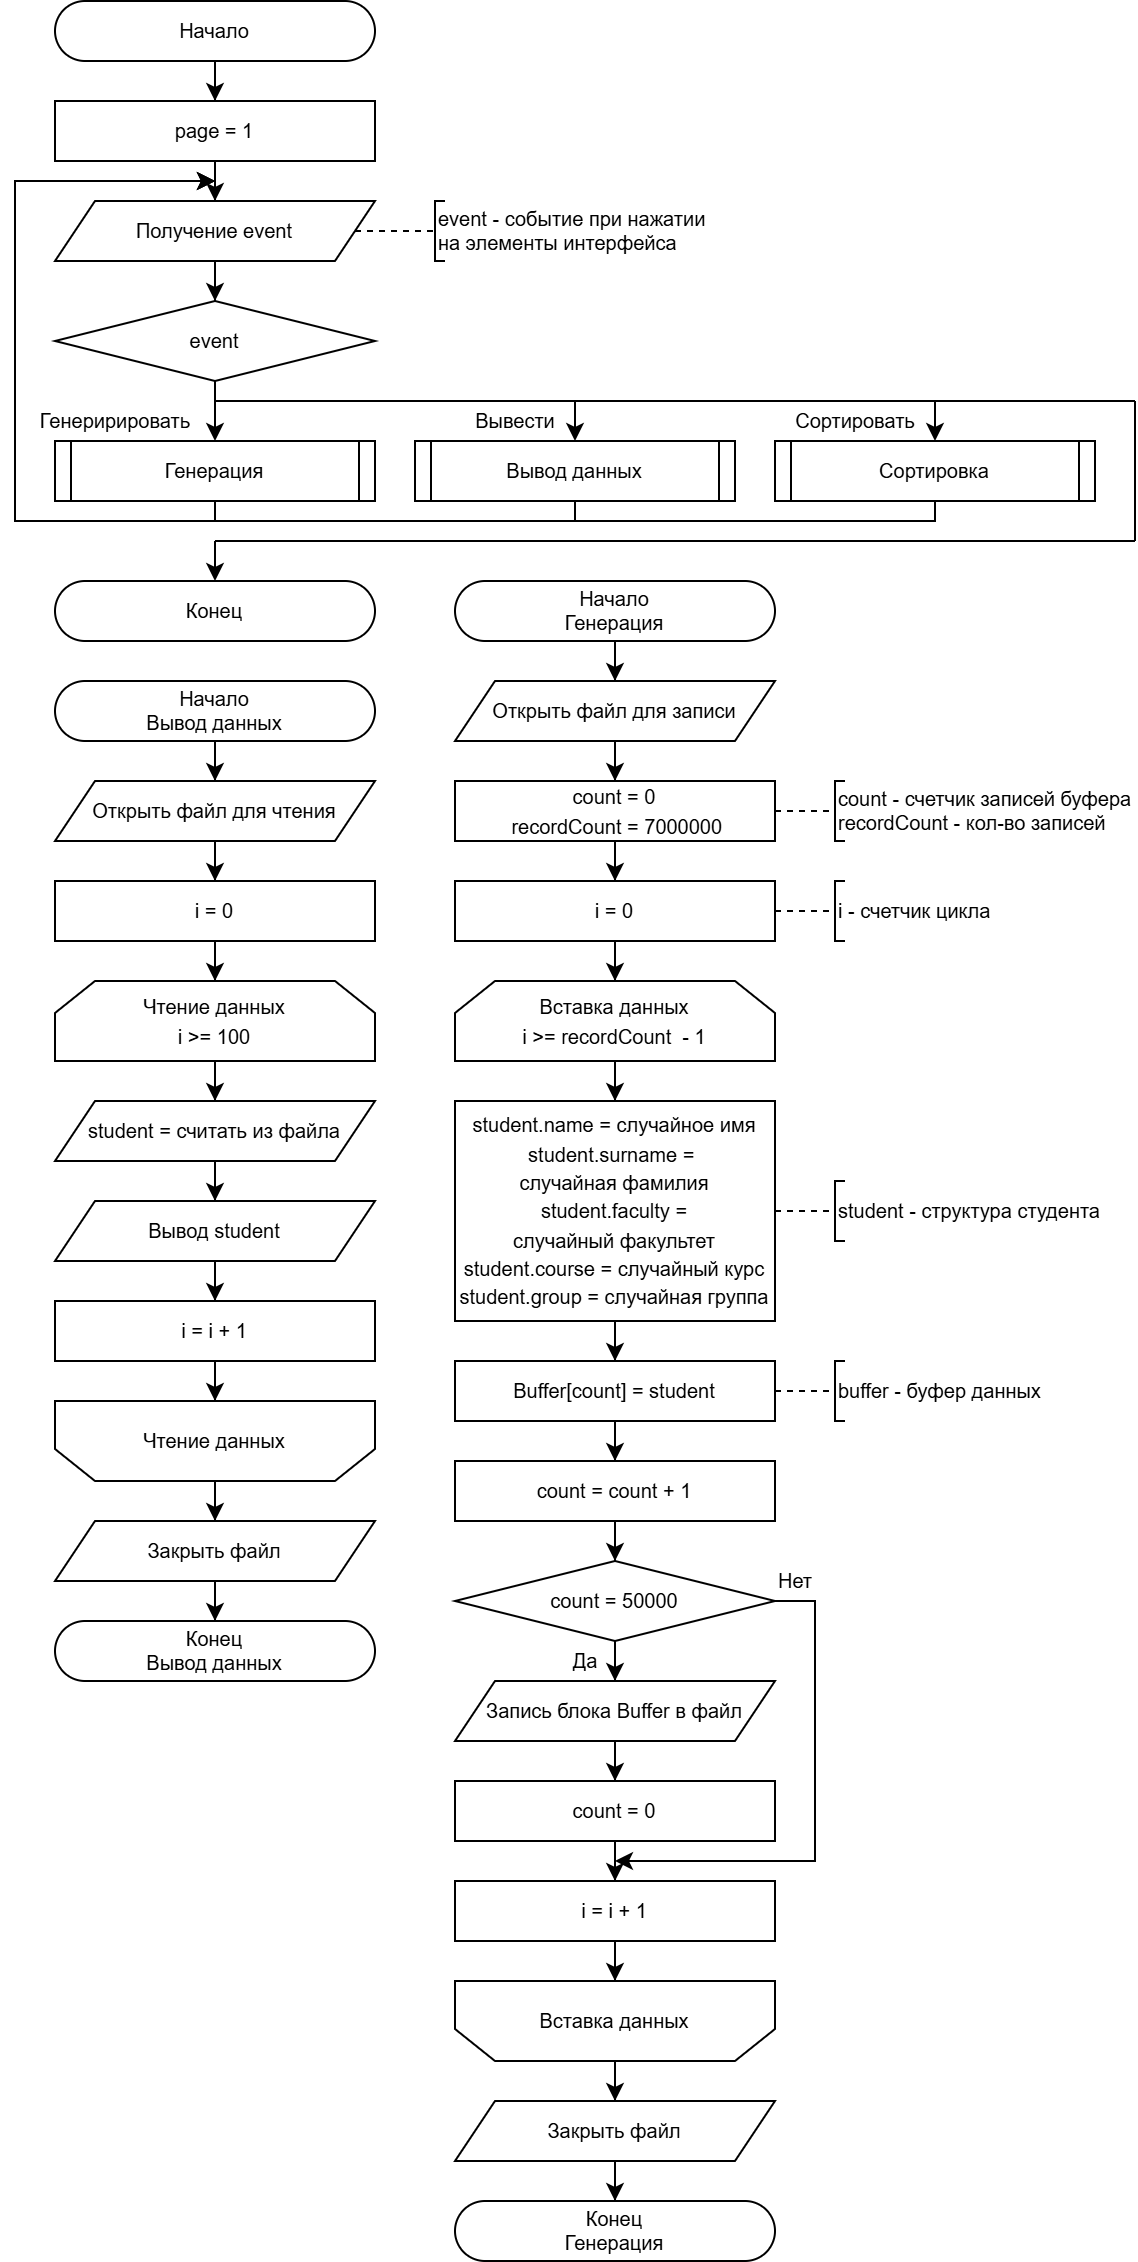
\includegraphics[width=0.592\linewidth]{images/s-1}
  \end{figure}
  \begin{center}
    Рисунок 1 – Схемы алгоритмов основной программы, генерации и вывода данных
  \end{center}

  \pagebreak

  \begin{figure}[h]
    \centering
    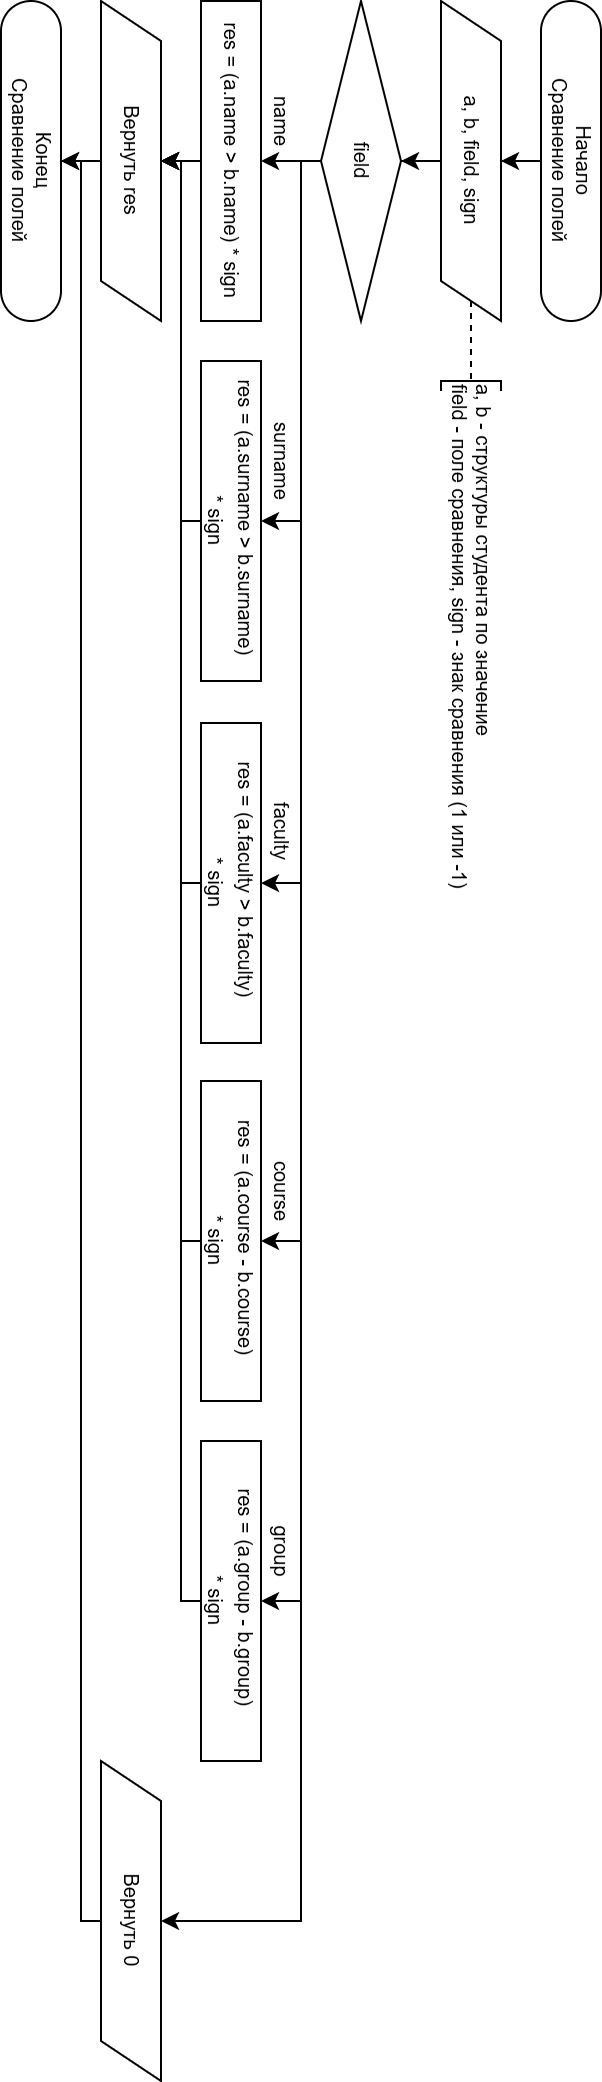
\includegraphics[width=0.3\linewidth]{images/s-2}
  \end{figure}
  \begin{center}
    Рисунок 2 – Схема алгоритма обработки событий
  \end{center}

  \pagebreak

  \begin{figure}[h]
    \centering
    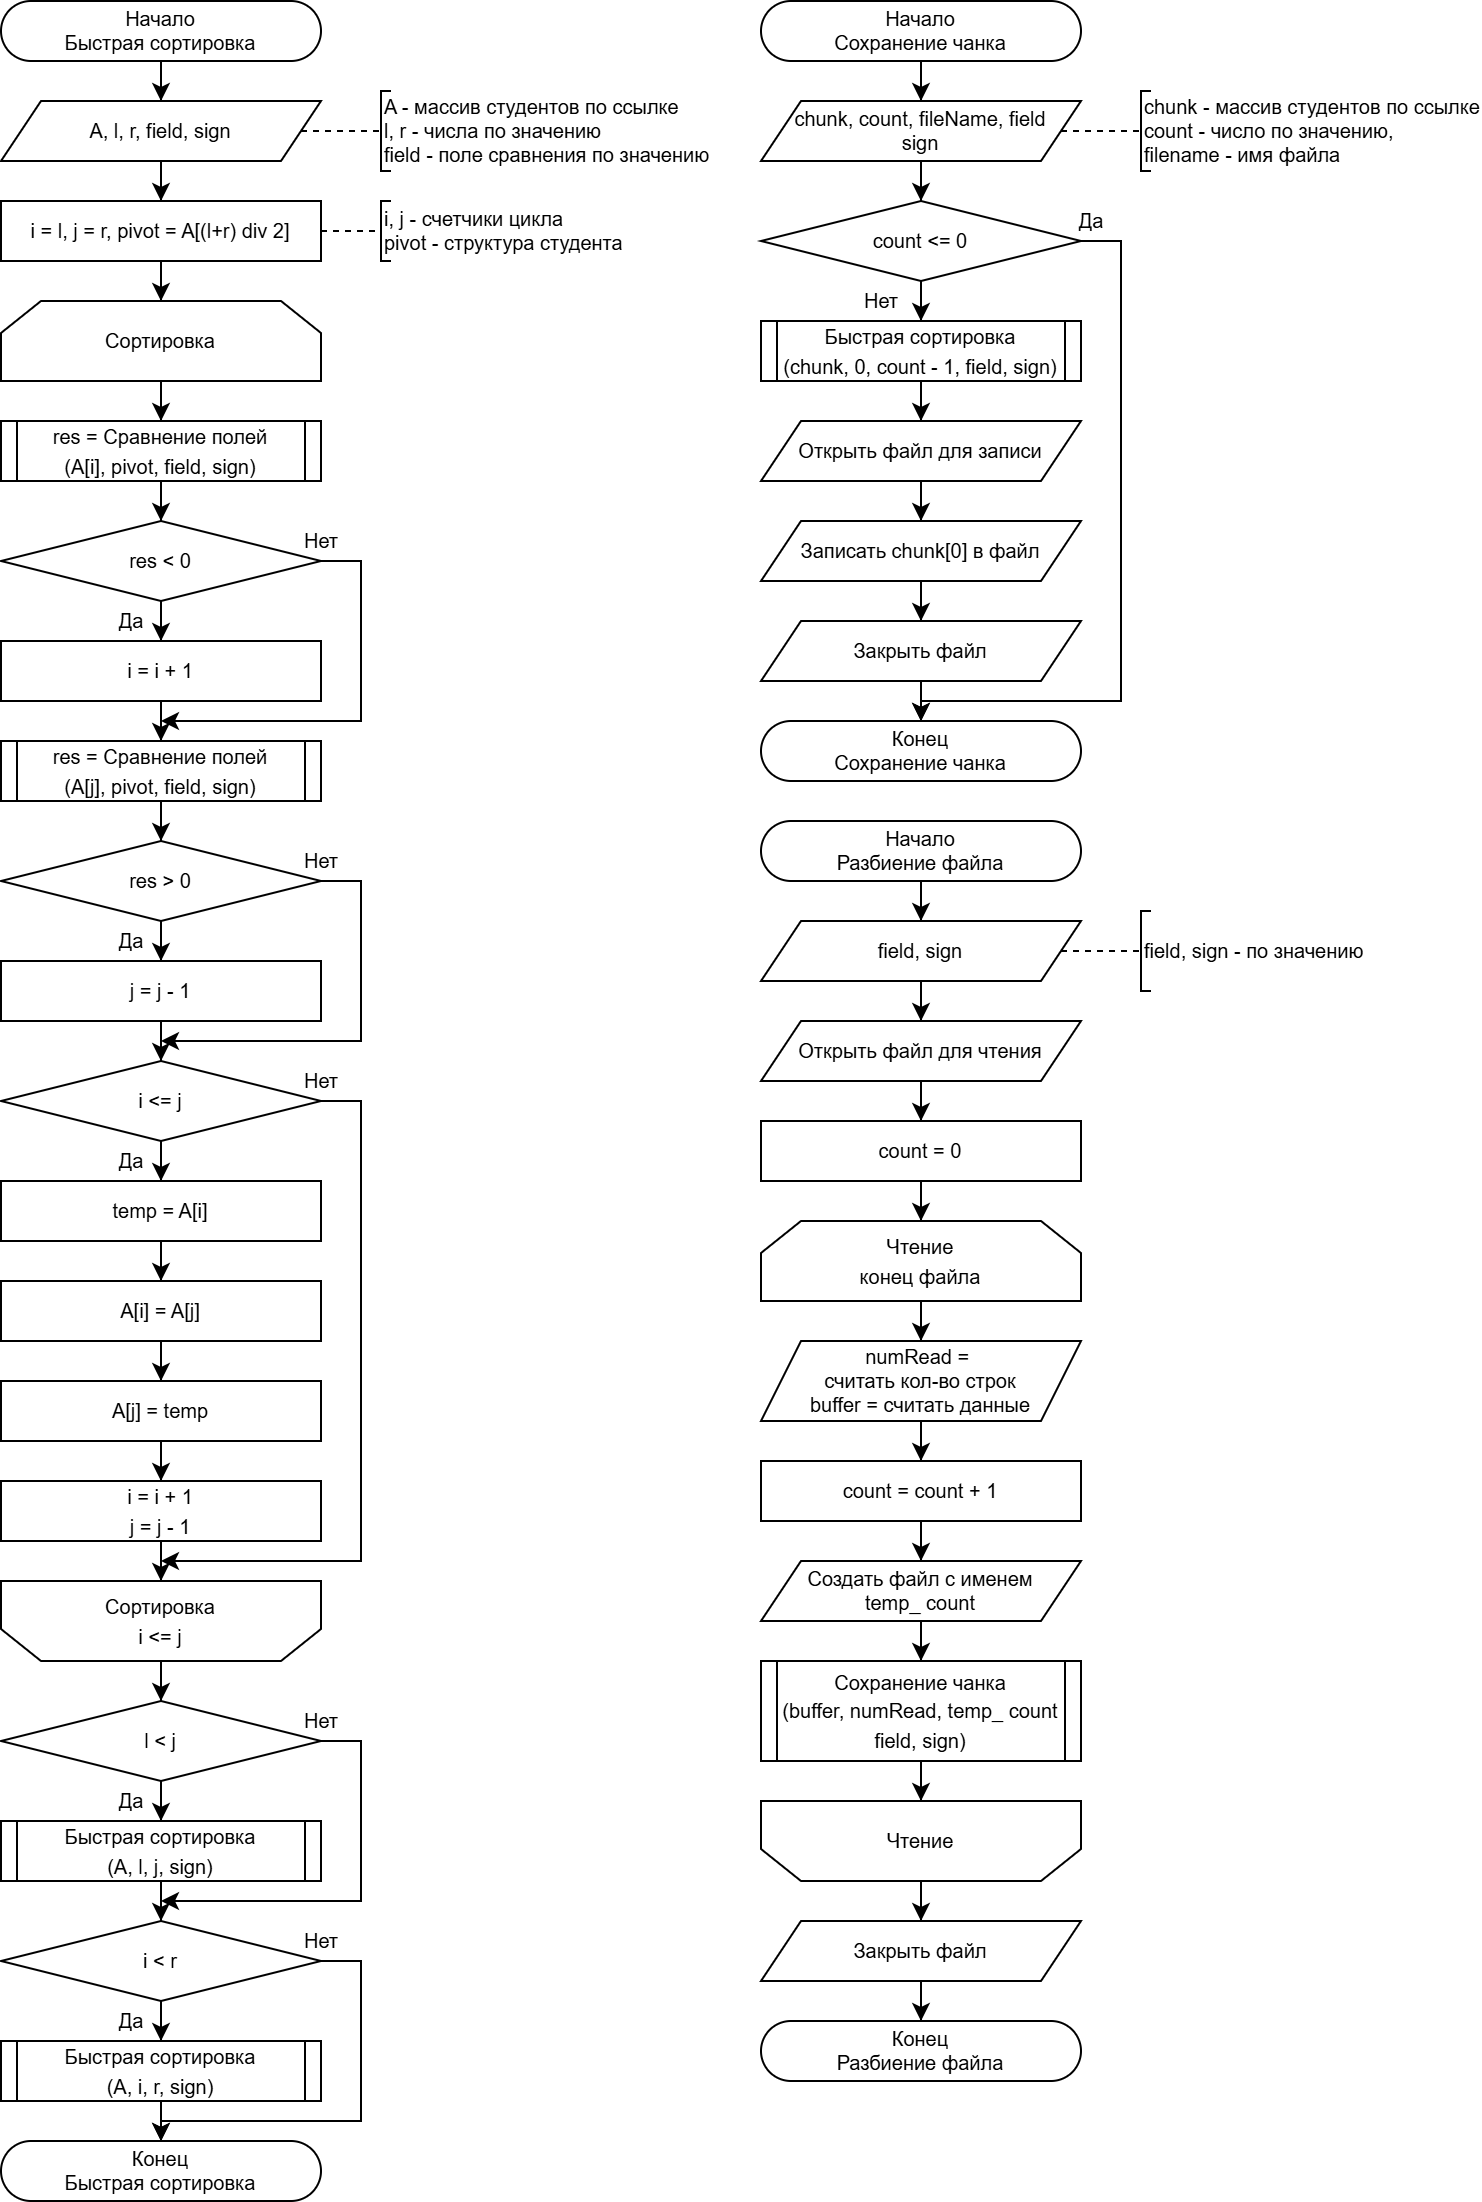
\includegraphics[width=0.79\linewidth]{images/s-3}
  \end{figure}
  \begin{center}
    Рисунок 3 – Схемы алгоритмов быстрой сортировки, сохранения чанка, разбиения файла
  \end{center}

  \pagebreak

  \begin{figure}[h]
    \centering
    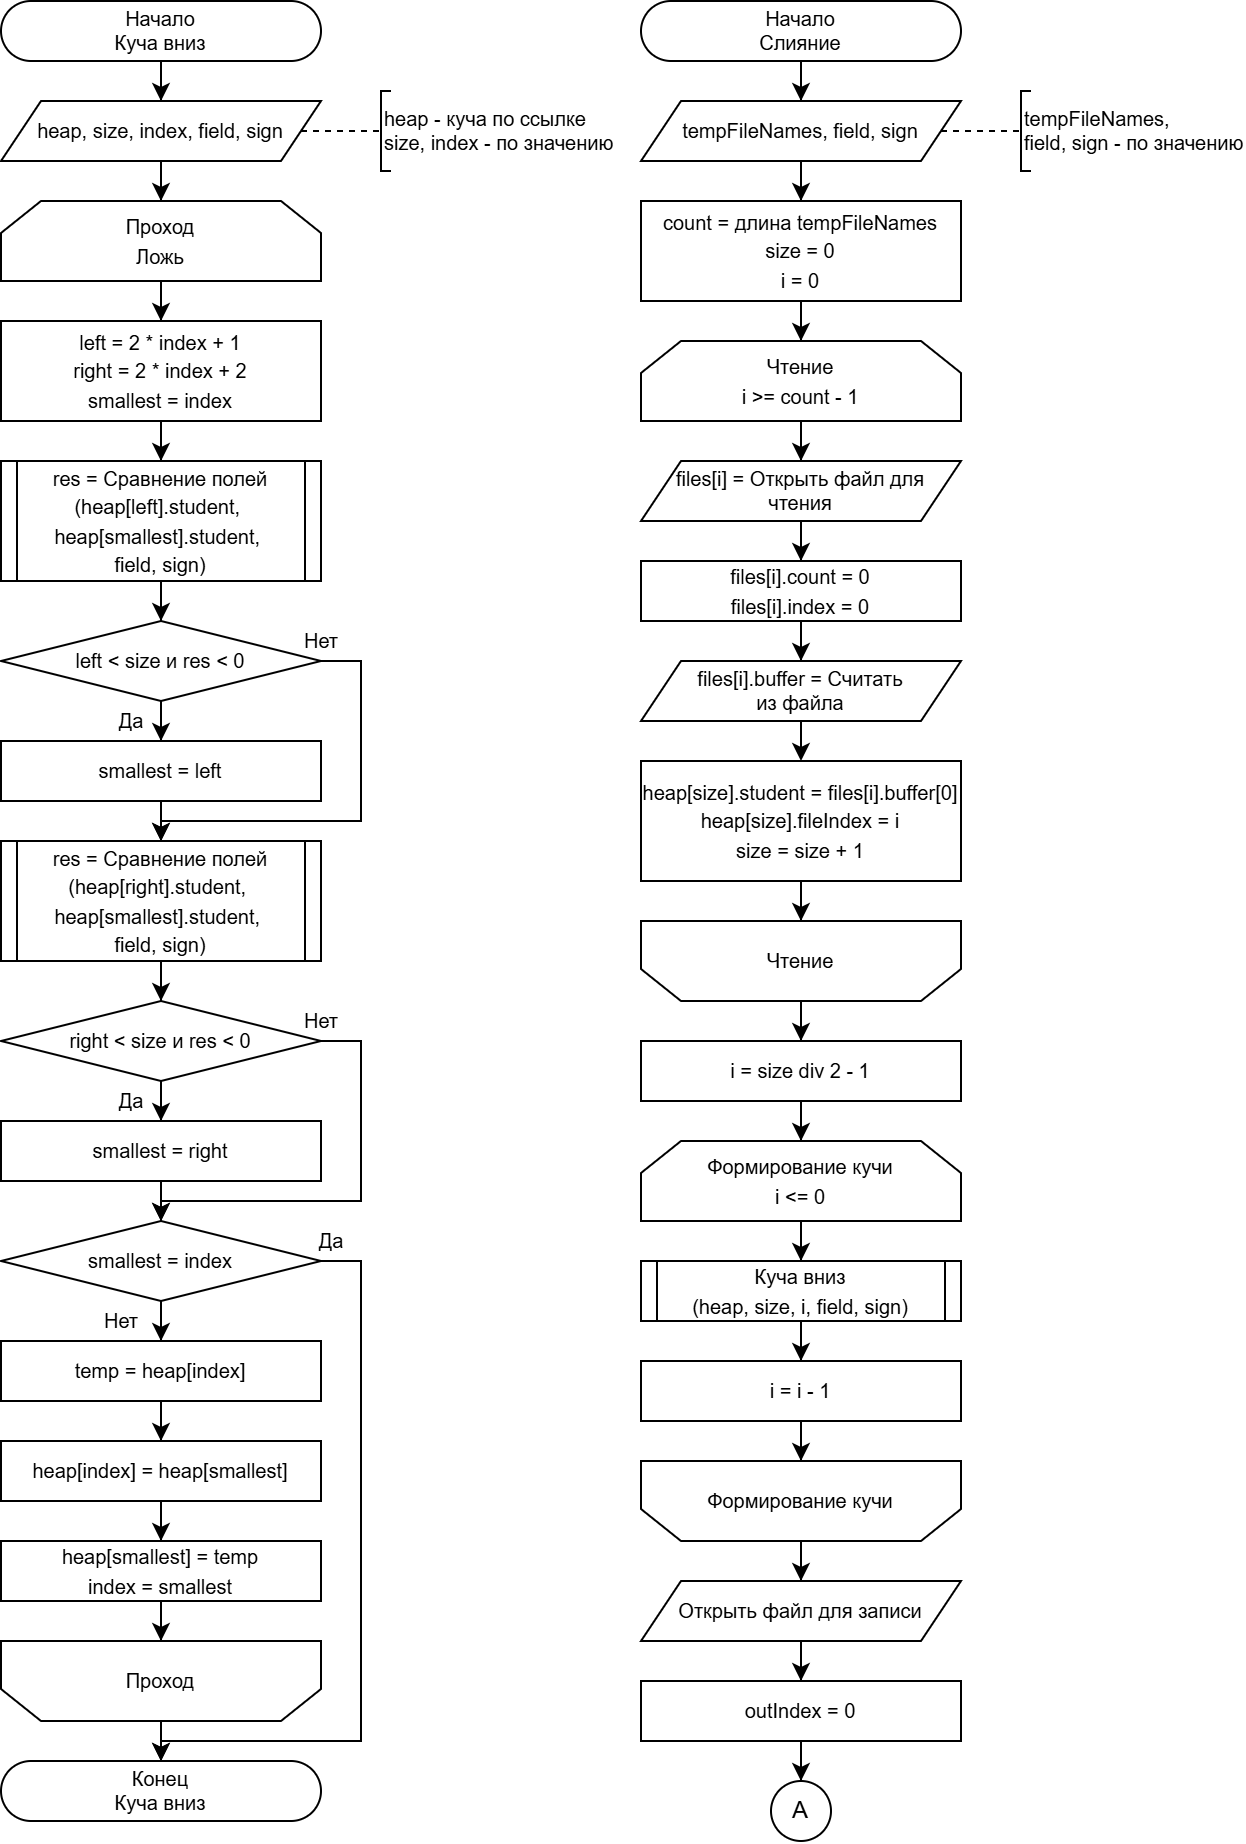
\includegraphics[width=0.79\linewidth]{images/s-5}
  \end{figure}
  \begin{center}
    Рисунок 4 – Схемы алгоритмов кучи вниз, слияния
  \end{center}

  \pagebreak

  \begin{figure}[h]
    \centering
    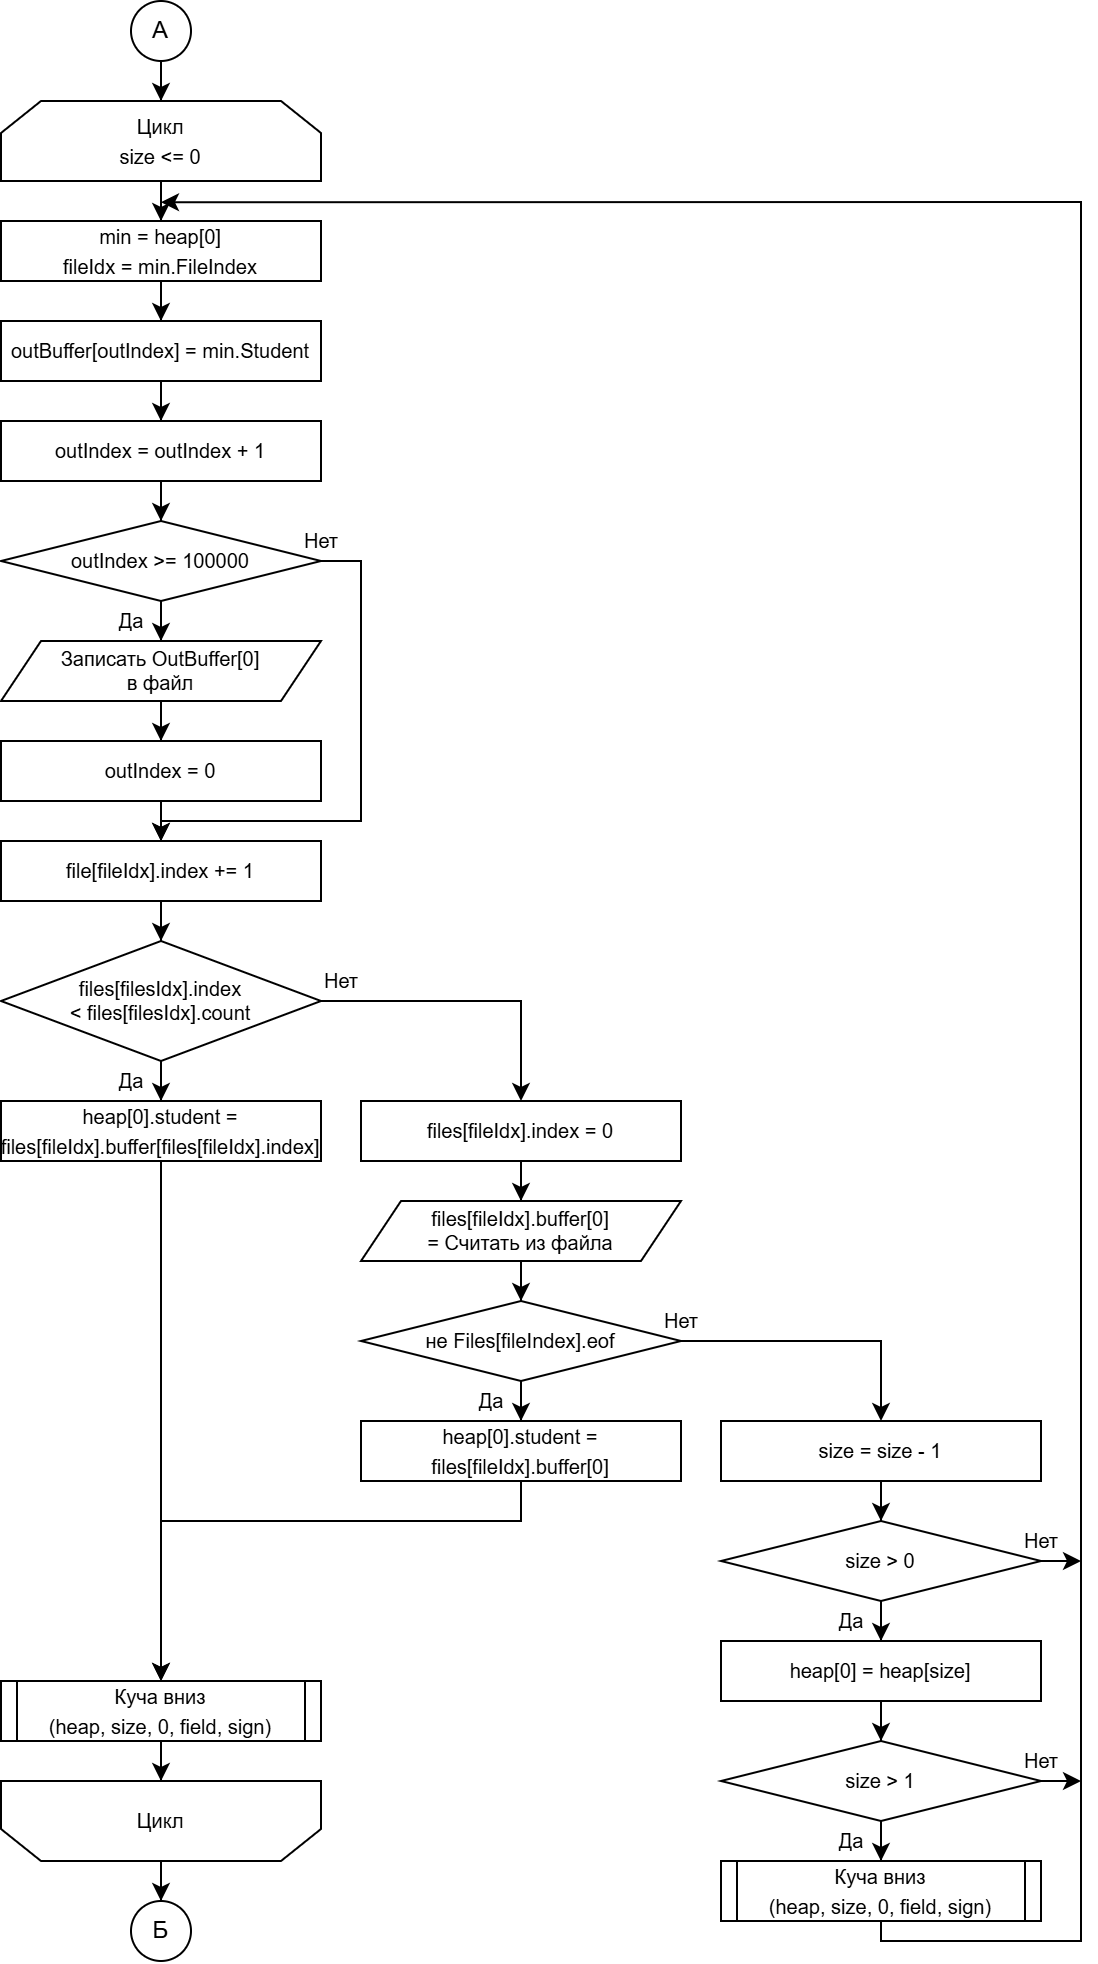
\includegraphics[width=0.65\linewidth]{images/s-6}
  \end{figure}
  \begin{center}
    Рисунок 5 – Продолжение схемы алгоритма слиения
  \end{center}

  \pagebreak

  \begin{figure}[h]
    \centering
    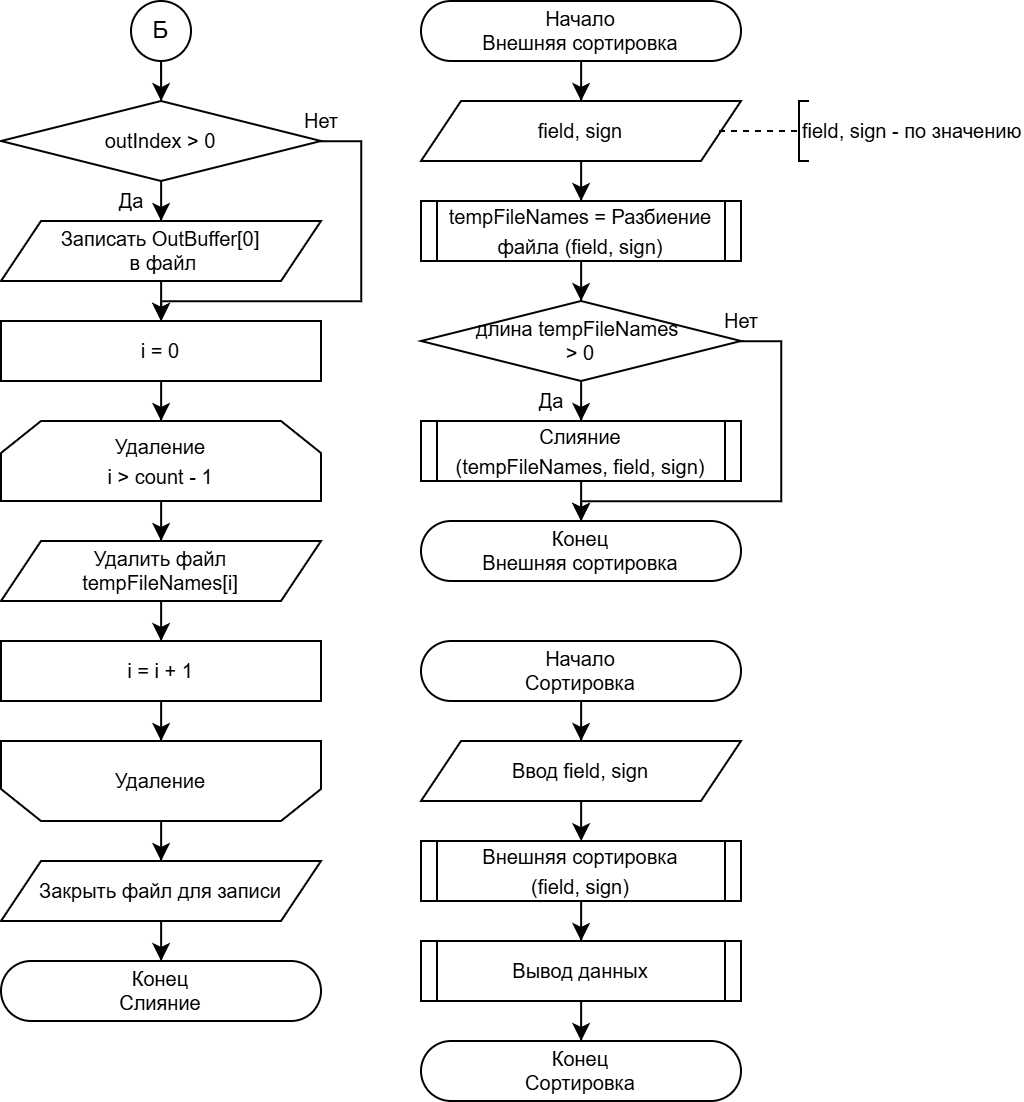
\includegraphics[width=0.7\linewidth]{images/s-7}
  \end{figure}
  \begin{center}
    Рисунок 6 – Продолжение схемы алгоритма слиения, схемы алгоритмов внешней сортировки, сортировки
  \end{center}

  Исходный код модуля программы на языке Pascal:

  \noindent
  \begin{Verbatim}[tabsize=4,fontsize=\small]
unit Unit1;

{$mode objfpc}{$H+}

interface

uses
  Classes, SysUtils, Forms, Controls, Graphics, Dialogs, StdCtrls, ExtCtrls,
  ComCtrls;

const
  RECORD_COUNT = 7000000;
  CHUNK_SIZE = 100000;
  BUF_SIZE = 100000;
  PAGE_SIZE = 100;

  NAMES: array[1..30] of string = (
    'Иван', 'Алексей', 'Сергей', 'Дмитрий', 'Андрей',
    'Александр', 'Михаил', 'Евгений', 'Максим', 'Артём',
    'Кирилл', 'Никита', 'Павел', 'Владимир', 'Илья',
    'Станислав', 'Роман', 'Георгий', 'Тимофей', 'Даниил',
    'Анна', 'Елена', 'Ольга', 'Наталья', 'Мария',
    'Екатерина', 'Анастасия', 'Виктория', 'Юлия', 'Дарья'
  );

  SURNAMES: array[1..20] of string = (
    'Петров', 'Смирнов', 'Иванов', 'Кузнецов', 'Попов',
    'Васильев', 'Новиков', 'Фёдоров', 'Морозов', 'Волков',
    'Алексеев', 'Лебедев', 'Семёнов', 'Егоров', 'Козлов',
    'Степанов', 'Николаев', 'Орлов', 'Андреев', 'Макаров'
  );

  FACULTIES: array[1..10] of string = (
    'Факультет технологий, инжиниринга и дизайна',
    'Факультет компьютерных и физико-математических наук',
    'Факультет автоматики и вычислительной техники',
    'Факультет экономики и финансов',
    'Факультет менеджмента и сервиса',
    'Факультет физической культуры и спорта',
    'Факультет педагогики и психологии',
    'Факультет истории, политических наук и культурологии',
    'Факультет филологии и медиакоммуникаций',
    'Факультет лингвистики'
  );

type
  TStudent = record
    name: string[40];
    surname: string[40];
    faculty: string[60];
    course: integer;
    group: integer;
  end;

  { TMainForm }

  TMainForm = class(TForm)
    ButtonNext: TButton;
    ButtonBack: TButton;
    ButtonSort: TButton;
    ButtonShow: TButton;
    ButtonGenerate: TButton;
    MemoRecords: TMemo;
    ProgressBar: TProgressBar;
    RadioButtonName: TRadioButton;
    RadioButtonSurname: TRadioButton;
    RadioButtonFaculty: TRadioButton;
    RadioButtonCourse: TRadioButton;
    RadioButtonGroup: TRadioButton;
    RadioButtonSortDown: TRadioButton;
    RadioButtonSortUp: TRadioButton;
    RadioGroupField: TRadioGroup;
    RadioGroupSort: TRadioGroup;
    procedure ButtonNextClick(Sender: TObject);
    procedure ButtonBackClick(Sender: TObject);
    procedure ButtonGenerateClick(Sender: TObject);
    procedure ButtonShowClick(Sender: TObject);
    procedure ButtonSortClick(Sender: TObject);
  private
    procedure ShowData;
    function CompareField(a, b: TStudent; field: string): integer;
    procedure QuickSort(var A: array of TStudent; l, r: integer; field: string);
    procedure SortAndSaveChunk(var Chunk: array of TStudent; count: Integer;
              fileName: string; field: string);
    function SplitInputFile(field: string): TStringArray;
    procedure MergeTempFiles(const TempFileNames: array of string;
              field: string);
    procedure ExternalMergeSort(field: string);
  public

  end;

var
  MainForm: TMainForm;
  page: integer = 1;

implementation

{$R *.lfm}

{ TMainForm }

procedure TMainForm.ButtonGenerateClick(Sender: TObject);
const
  BUF_WRITE_SIZE = 50000;
var
  dataFile: file of TStudent;
  student: TStudent;
  i, count, numWritten: integer;
  Buffer: array of TStudent;
begin
  Randomize;
  AssignFile(dataFile, 'data.dat');
  Rewrite(dataFile);
  SetLength(Buffer, BUF_WRITE_SIZE);

  ProgressBar.Position := 0;
  count := 0;

  for i := 0 to RECORD_COUNT - 1 do
  begin
    student.name := NAMES[Random(Length(NAMES)) + 1];
    student.surname := SURNAMES[Random(Length(SURNAMES)) + 1];
    student.faculty := FACULTIES[Random(Length(FACULTIES)) + 1];
    student.course := Random(4) + 1;
    student.group := 1000 + Random(1000);

    Buffer[count] := student;
    count := count + 1;

    if count = BUF_WRITE_SIZE then
    begin
      BlockWrite(dataFile, Buffer[0], count, numWritten);
      count := 0;
      ProgressBar.Position := Round((i * 100) / RECORD_COUNT);
    end;
  end;

  CloseFile(dataFile);
  SetLength(Buffer, 0);
  ProgressBar.Position := 100;
end;

procedure TMainForm.ShowData;
var
  dataFile: file of TStudent;
  student: TStudent;
  i: integer;
begin
  AssignFile(dataFile, 'data.dat');
  Reset(dataFile);
  MemoRecords.Clear;
  ProgressBar.Position := 0;

  for i := (page - 1) * PAGE_SIZE to page * PAGE_SIZE - 1 do
  begin
    Seek(dataFile, i);
    Read(dataFile, student);

    MemoRecords.Lines.Add(
      Format('%d. %s %s, %s, курс: %d, группа: %d',
        [i + 1, student.surname, student.name, student.faculty,
          student.course, student.group])
    );

    ProgressBar.Position := Round((i - (page - 1) * 
                            PAGE_SIZE) * 100 / PAGE_SIZE);
  end;

  CloseFile(dataFile);
  ProgressBar.Position := 100;
end;

procedure TMainForm.ButtonBackClick(Sender: TObject);
begin
  if page > 1 then
  begin
    page := page - 1;
    ShowData;
  end;
end;

procedure TMainForm.ButtonNextClick(Sender: TObject);
begin
  if page <> RECORD_COUNT div PAGE_SIZE then
  begin
    page := page + 1;
    ShowData;
  end;
end;

procedure TMainForm.ButtonShowClick(Sender: TObject);
begin
  ShowData;
end;

function TMainForm.CompareField(a, b: TStudent; field: string): integer;
var
  sign: integer;
begin
  if RadioButtonSortUp.Checked then
    sign := 1
  else
    sign := -1;

  case field of
    'name': Result := sign * CompareStr(a.name, b.name);
    'surname': Result := sign * CompareStr(a.surname, b.surname);
    'faculty': Result := sign * CompareStr(a.faculty, b.faculty);
    'course': Result := sign * (a.course - b.course);
    'group': Result := sign * (a.group - b.group);
    else Result := 0;
  end;
end;

procedure TMainForm.QuickSort(var A: array of TStudent;
                              l, r: integer; field: string);
var
  i, j: Integer;
  pivot, temp: TStudent;
begin
  if r - l < 1 then Exit;

  i := l;
  j := r;
  pivot := A[(l + r) div 2];

  repeat
    while CompareField(A[i], pivot, field) < 0 do i := i + 1;
    while CompareField(A[j], pivot, field) > 0 do j := j - 1;

    if i <= j then
    begin
      temp := A[i];
      A[i] := A[j];
      A[j] := temp;
      i := i + 1;
      j := j - 1;
    end;
  until i > j;

  if l < j then QuickSort(A, l, j, field);
  if i < r then QuickSort(A, i, r, field);
end;

procedure TMainForm.SortAndSaveChunk(var Chunk: array of TStudent;
          count: Integer; fileName: string; field: string);
var
  tempFile: file of TStudent;
begin
  if count <= 0 then Exit;

  QuickSort(Chunk, 0, count - 1, field);
  AssignFile(tempFile, fileName);
  Rewrite(tempFile);
  BlockWrite(tempFile, Chunk[0], count);
  CloseFile(tempFile);
end;

function TMainForm.SplitInputFile(field: string): TStringArray;
var
  dataFile: file of TStudent;
  Buffer: array of TStudent;
  count, numRead: integer;
begin
  SetLength(Result, 0);

  AssignFile(dataFile, 'data.dat');
  Reset(dataFile);
  SetLength(Buffer, CHUNK_SIZE);
  count := 0;

  while not Eof(dataFile) do
  begin
    BlockRead(dataFile, Buffer[0], CHUNK_SIZE, numRead);
    if numRead > 0 then
    begin
      count := count + 1;
      SetLength(Result, count);
      Result[count - 1] := 'temp_' + IntToStr(count) + '.dat';
      SortAndSaveChunk(Buffer, numRead, Result[count - 1], field);
    end;
  end;

  CloseFile(dataFile);
  SetLength(Buffer, 0);
end;

procedure TMainForm.MergeTempFiles(const TempFileNames: array of string; 
                                    field: string);
type
  TFileBuffer = record
    FileHandle: file of TStudent;
    Buffer: array of TStudent;
    Count, Index: Integer;
    Eof: Boolean;
  end;

  THeapItem = record
    Student: TStudent;
    FileIndex: Integer;
  end;

  procedure HeapifyDown(var Heap: array of THeapItem; size: Integer; 
                        index: Integer);
  var
    left, right, smallest: Integer;
    temp: THeapItem;
  begin
    while True do
    begin
      left := 2 * index + 1;
      right := 2 * index + 2;
      smallest := index;

      if (left < size) and
         (CompareField(Heap[left].Student, 
         Heap[smallest].Student, field) < 0) then
        smallest := left;

      if (right < size) and
         (CompareField(Heap[right].Student, 
         Heap[smallest].Student, field) < 0) then
        smallest := right;

      if smallest = index then Break;

      temp := Heap[index];
      Heap[index] := Heap[smallest];
      Heap[smallest] := temp;
      index := smallest;
    end;
  end;

var
  Files: array of TFileBuffer;
  OutBuffer: array of TStudent;
  OutIndex, filesCount: Integer;
  dataFile: file of TStudent;
  Heap: array of THeapItem;
  HeapSize: Integer;
  i, fileIdx: Integer;
  minItem: THeapItem;
begin
  filesCount := Length(TempFileNames);
  if filesCount = 0 then Exit;

  SetLength(Files, filesCount);
  SetLength(Heap, filesCount);
  HeapSize := 0;

  for i := 0 to filesCount - 1 do
  begin
    AssignFile(Files[i].FileHandle, TempFileNames[i]);
    Reset(Files[i].FileHandle);
    SetLength(Files[i].Buffer, BUF_SIZE);
    Files[i].Count := 0;
    Files[i].Index := 0;
    BlockRead(Files[i].FileHandle, Files[i].Buffer[0], 
              BUF_SIZE, Files[i].Count);
    Files[i].Eof := (Files[i].Count = 0) or (Ioresult <> 0);

    if not Files[i].Eof then
    begin
      Heap[HeapSize].Student := Files[i].Buffer[0];
      Heap[HeapSize].FileIndex := i;
      Inc(HeapSize);
    end;
  end;

  for i := HeapSize div 2 - 1 downto 0 do
    HeapifyDown(Heap, HeapSize, i);

  SetLength(OutBuffer, BUF_SIZE);
  OutIndex := 0;
  AssignFile(dataFile, 'data.dat');
  Rewrite(dataFile);

  while HeapSize > 0 do
  begin
    min := Heap[0];
    fileIdx := min.FileIndex;

    OutBuffer[OutIndex] := min.Student;
    Inc(OutIndex);

    if OutIndex >= BUF_SIZE then
    begin
      BlockWrite(dataFile, OutBuffer[0], OutIndex);
      OutIndex := 0;
    end;

    Inc(Files[fileIdx].Index);

    if Files[fileIdx].Index < Files[fileIdx].Count then
    begin
      Heap[0].Student := Files[fileIdx].Buffer[Files[fileIdx].Index];
    end
    else
    begin
      Files[fileIdx].Index := 0;
      BlockRead(Files[fileIdx].FileHandle, Files[fileIdx].Buffer[0], BUF_SIZE, 
                Files[fileIdx].Count);
      Files[fileIdx].Eof := (Files[fileIdx].Count = 0) or (Ioresult <> 0);

      if not Files[fileIdx].Eof then
      begin
        Heap[0].Student := Files[fileIdx].Buffer[0];
      end
      else
      begin
        Dec(HeapSize);
        if HeapSize > 0 then
        begin
          Heap[0] := Heap[HeapSize];

          if HeapSize > 1 then
            HeapifyDown(Heap, HeapSize, 0);
        end;
        Continue;
      end;
    end;

    if HeapSize > 1 then
      HeapifyDown(Heap, HeapSize, 0);
  end;

  if OutIndex > 0 then
    BlockWrite(dataFile, OutBuffer[0], OutIndex);

  for i := 0 to filesCount - 1 do
  begin
    CloseFile(Files[i].FileHandle);
    if FileExists(TempFileNames[i]) then
      DeleteFile(TempFileNames[i]);
  end;

  CloseFile(dataFile);

  SetLength(Files, 0);
  SetLength(Heap, 0);
  SetLength(OutBuffer, 0);
end;

procedure TMainForm.ExternalMergeSort(field: string);
var
  TempFileNames: TStringArray;
begin
  TempFileNames := SplitInputFile(field);

  if Length(TempFileNames) > 0 then
    MergeTempFiles(TempFileNames, field);

  SetLength(TempFileNames, 0);
end;

procedure TMainForm.ButtonSortClick(Sender: TObject);
begin
  if RadioButtonName.Checked then ExternalMergeSort('name');
  if RadioButtonSurname.Checked then ExternalMergeSort('surname');
  if RadioButtonFaculty.Checked then ExternalMergeSort('faculty');
  if RadioButtonCourse.Checked then ExternalMergeSort('course');
  if RadioButtonGroup.Checked then ExternalMergeSort('group');

  ShowData();
end;

end.
  \end{Verbatim}

  \section*{Вывод}
  В ходе лабораторной работы была разработана программа с графическим интерфейсом для внешней сортировки файлов, что позволило освоить алгоритмы многопутевого слияния и работу с файлами в Lazarus.

\end{document}